%Dokumentklasse
\documentclass[a4paper,12pt,parskip=full]{scrreprt}
\usepackage[left= 2.5cm,right = 2cm, bottom = 4 cm]{geometry}
%\usepackage[onehalfspacing]{setspace}
% ============= Packages =============

% Dokumentinformationen
\usepackage[
	pdftitle={Physik basierter Charaktercontroller mit Unity Machine Learning},
	pdfsubject={},
	pdfauthor={Simon Grözinger},
	pdfkeywords={},	
	%Links nicht einrahmen
	hidelinks
]{hyperref}


% Standard Packages
\usepackage[utf8]{inputenc}
\usepackage[ngerman]{babel}
\usepackage[T1]{fontenc}
\usepackage{graphicx, subfig}
\graphicspath{{img/}}
\usepackage{fancyhdr}
\usepackage{lmodern}
\usepackage{color}
\usepackage{enumitem}

% Extra Packages
\usepackage{float}
\usepackage[table]{xcolor}
\usepackage{listings}
\lstset{
language=[Sharp]C,
captionpos=b,
numbers=left, %Nummerierung
frame=single, % Oberhalb und unterhalb des Listings ist eine Linie
showspaces=false,
showtabs=false,
breaklines=true,
showstringspaces=false,
breakatwhitespace=true,
escapeinside={(*@}{@*)},
commentstyle=\color{greencomments},
morekeywords={partial, var, value, get, set},
keywordstyle=\color{bluekeywords},
stringstyle=\color{redstrings},
basicstyle=\ttfamily\small,
literate=%
  {Ö}{{\"O}}1
  {Ä}{{\"A}}1
  {Ü}{{\"U}}1
  {ß}{{\ss}}1
  {ü}{{\"u}}1
  {ö}{{\"o}}1
  {ä}{{\"a}}1
  }
  
\definecolor{bluekeywords}{rgb}{0,0,1}
\definecolor{greencomments}{rgb}{0,0.5,0}
\definecolor{redstrings}{rgb}{0.64,0.08,0.08}
\definecolor{xmlcomments}{rgb}{0.5,0.5,0.5}
\definecolor{types}{rgb}{0.17,0.57,0.68}

% ============= BibLatex =============
\usepackage[backend=bibtex,style=numeric]{biblatex}
%Literaturverzeichnis
\addbibresource{Literatur.bib}

% ============= Remove new Page =============
\usepackage{etoolbox}
\makeatletter
\patchcmd{\chapter}{\if@openright\cleardoublepage\else\clearpage\fi}{}{}{}
\makeatother

% zusätzliche Schriftzeichen der American Mathematical Society
\usepackage{amsfonts}
\usepackage{amsmath}

%nicht einrücken nach Absatz
%\setlength{\parindent}{0pt}


% ============= Kopf- und Fußzeile =============
\pagestyle{fancy}
%
\lhead{}
\chead{}
\rhead{\slshape \leftmark}
%%
\lfoot{}
\cfoot{\thepage}
\rfoot{}
%%
\renewcommand{\headrulewidth}{0.4pt}
\renewcommand{\footrulewidth}{0pt}

% ============= Package Einstellungen & Sonstiges ============= 
%Besondere Trennungen
\hyphenation{De-zi-mal-tren-nung}


% ============= Dokumentbeginn =============

\begin{document}
%Seiten ohne Kopf- und Fußzeile sowie Seitenzahl
\pagestyle{empty}

\begin{center}
\begin{tabular}{p{\textwidth}}


\begin{flushright}

\includegraphics[scale=0.1]{img/logos.jpg}
\end{flushright}


\\

\begin{center}
\LARGE{\textsc{
Entwicklung eines physikbasierten Charaktercontrollers mit Unity ML Agents\\
}}
\end{center}

\\


\begin{center}
\large{\textbf{Software-Engineering}\\}
\large{Fakultät für Informatik \\
der Hochschule Heilbronn \\}
\end{center}

\\

\begin{center}
\textbf{\Large{Bachelor-Thesis}}
\end{center}

\begin{center}
vorgelegt von
\end{center}

\begin{center}
\large{\textbf{Simon Grözinger}} \\
\small{Matrikelnummer: 205047} \\
\end{center}

\end{tabular}
\end{center}

%Inhaltsverzeichnis
\tableofcontents

%Abbildungsverzeichnis
\listoffigures

% pagestyle für gesamtes Dokument aktivieren
\pagestyle{fancy}

\chapter{Einleitung}
\label{sec:einleitung}
Seit einigen Jahren steigt die Präsenz von AI und somit maschinellem Lernen in unserem Alltag. Systeme wie ChatGPT sind nicht mehr wegzudenken. Ein interessantes Feld ist dabei auch die Steuerung von Robotern, speziell humanoiden Robotern. Die Roboter werden vorab meist in einer virtuellen Trainingsumgebung trainiert, um negative Auswirkungen wie Maschinenschaden zu verhindern und gleichzeitig die Notwendigkeit für die teure Anschaffung mehrerer Roboter zu vermeiden. Der Schritt zur Verwendung ähnlicher Systeme in der Videospielbranche ist daher nicht weit entfernt.

Nvidia und Ubisoft zeigen schon seit 2020 Prototypen zur Verwendung von maschinellem Lernen im Prozess der Charaktersteuerung bzw. Charakteranimation.\cite{2022-TOG-ASE}\cite{10.1145/3355089.3356536} Im Fall von Ubisoft wird klar gezeigt, welche Komplexität das Animationssystem ihrer top Titel aufweist. Maschinelles Lernen ermöglicht die Reduktion dieser Systeme in antrainierten Modellen. Speziell die Verwendung von physikalisch simulierten Charakteren ermöglicht einen Lernprozess vergleichbar mit dem eines Menschen.

Ziel der Arbeit ist es, einen Charakter physikalisch in der Unity Spieleumgebung zu simulieren. Der Charakter soll mit maschinellen Lernverfahren darauf trainiert werden, das Gleichgewicht zu halten und sich zu einem Ziel zu bewegen. Als Basis für die Trainingsumgebung soll die im Unity ML-Agents Framework entwickelte Walker Demo zum Einsatz kommen. Die Demo soll erweitert werden, sodass der Walker über Tastatureingaben gesteuert und somit in Videospielen als Ersatz für traditionelle Animationssysteme verwendet werden kann. Um die Vielfalt von Charakteranimationen abzudecken wird analysiert, wie weitere Bewegungsabläufe in das bestehende System eingefügt werden können. Außerdem soll auch die Kompatibilität mit unterschiedlichen Charaktermodellen geprüft werden.

Zu Beginn wird im Kapitel Grundlagen das Teilgebiet \grqq{}Verstärkendes Lernen\grqq{} aus dem Fachgebiet maschinelles Lernen erklärt. Darauf aufbauend werden anschließend der Aufbau, die Komponenten und Implementierungsschnittstellen der Unity ML-Agents Library aufgezeigt. Abgeschlossen werden die Grundlagen mit einer Übersicht der für die Simulation verwendeten Physikkomponenten in Unity. Auf die Grundlagen folgt eine Analyse der Walker Demo. Die Walker Demo ist eine Trainingsumgebung, welche innerhalb des Unity ML-Agents Projekts zur Demonstration der Fähigkeiten der Library entwickelt wurde. Im weiteren Verlauf der Arbeit dient diese Demonstration als Basis für den entwickelten Charaktercontroller. In Kapitel 4 wird näher auf die Entwicklung, die ausgeführten Versuchen sowie die darauf folgenden Ergebnisse eingegangen. Kapitel 4 teilt sich dabei in 4 Teile. In Teil 1 wird die Nutzersteuerung thematisiert. Teil 2 ermittelt, welche Anpassungen am Trainingsablauf gemacht werden müssen, um gängige Bewegungsabläufe eines Videospiel-Charakters zu ermöglichen. In Teil 3 - Charakterkompatibilität und Konfiguration - werden die Komponenten der Demo angepasst, um die Konfiguration zu vereinfachen, sowie das Steuern von unterschiedlichen Charaktermodellen zu gewährleisten. Teil 4 analysiert Anpassungen, um das erlernte Gangbild natürlicher zu gestalten. Abschließend werden in Zusammenfassung und Ausblick die in der Arbeit umgesetzten Prototypen auf ihre Anwendbarkeit in Videospielen analysiert und ein Ausblick für weitere Forschungen sowie bereits existierende Forschungen in anderen Softwareumgebungen aus diesem Bereich aufgezeigt.
{\chapter{Verstärkendes Lernen}}
\label{sec:rl}
Der Begriff 'Verstärkendes Lernen' beschreibt eine Art von Problemstellung und die dafür geeigneten Problemlösungsmethoden im Bereich des Maschinellen Lernens. Die grundlegenden Bestandteile einer Trainingsumgebung sind der Agent und die Umgebung, in der der Agent seine Aktionen ausführt. Der Ansatz ist in vielerlei Hinsicht vergleichbar mit dem Lernvorgang von Menschen. Ein Baby lernt das Krabbeln ohne direkte Anweisungen, nur durch die Wahrnehmung der Umgebung, das Verhalten der Umgebung in Relation zu seinen Bewegungen und die mit den Bewegungen einhergehenden Belohnungen. Auf dieselbe Art lernt der Agent beim Verstärkenden Lernen von jedem Zustand die Aktion auszuführen, um die Belohnung zu maximieren. Im Fall des Babys sind die Belohnungen Faktoren wie Schmerz, Hunger, Müdigkeit oder gestillte Neugier. Der Agent hingegen erhält eine numerische Belohnung.\cite{sutton2018reinforcement}

\begin{figure}[htb]
  \centering  
  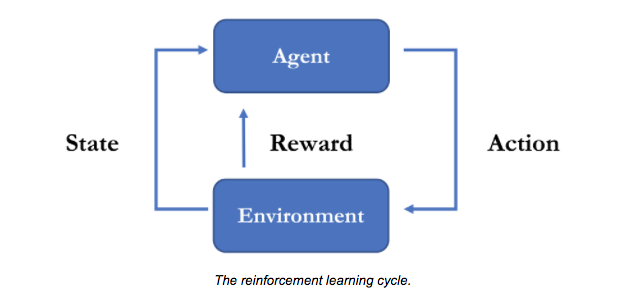
\includegraphics[scale=0.5]{img/rl_cycle.png}
  \caption{Verstärkendes Lernen Ablauf \protect\cite{unity_mlagents_rl_cycle}}
  \label{fig:rl_cycle}
\end{figure}

Die Abbildung 2.1 zeigt die Verbindungen zwischen dem Agent und der Umgebung. Der Agent erhält als Input einen Zustand oder meist einen Teilzustand der Umgebung und reagiert darauf mit einer Aktion. Dieser Zyklus kann je nach Problem in unterschiedlichen Intervallen durchlaufen werden. Bei kontinuierlichen Kontrollproblemen werden Aktionen meist in regelmäßigen Intervallen abgefragt. Bei rundenbasierten Spielen kann dieser Vorgang jedoch auch nur einmal pro Runde stattfinden.
{\chapter{PPO}}
\label{sec:ppo}
Das Unity ML-Agents Packet beinhaltet zwei bereits implementierte Algorithmen, SAC (Soft Actor Critic) und PPO (Proximal Policy Optimization). Beim testen der Walker Demo mit den zwei Algorithmen waren die Endergebnisse vergleichbar.
Jedoch hat der SAC Algorithmus in dieser Umgebung mehr Zeit gebraucht und das Lernverhalten war instabiler. Daher wird in der Arbeit der PPO Algorithmus von Open Ai verwendet. In diesem Kapitel wird die Funktionsweise hinter dem Algorithmus näher erklärt.

Der PPO Algorithmus basiert auf dem Akteur Kritik (Actor Critic) Ansatz. Der Akteur Kritik Ansatz nutz zwei neuronale Netze, das Akteur Netz lernt die Zuordnung von Zustand zu Aktion während das Kritik Netz bewertet wie gut es ist die Aktion zu wählen basierend auf dem aktuellen Zustand.

Akteur Verlust Funktion:
\begin{figure}[H]
  \centering  
  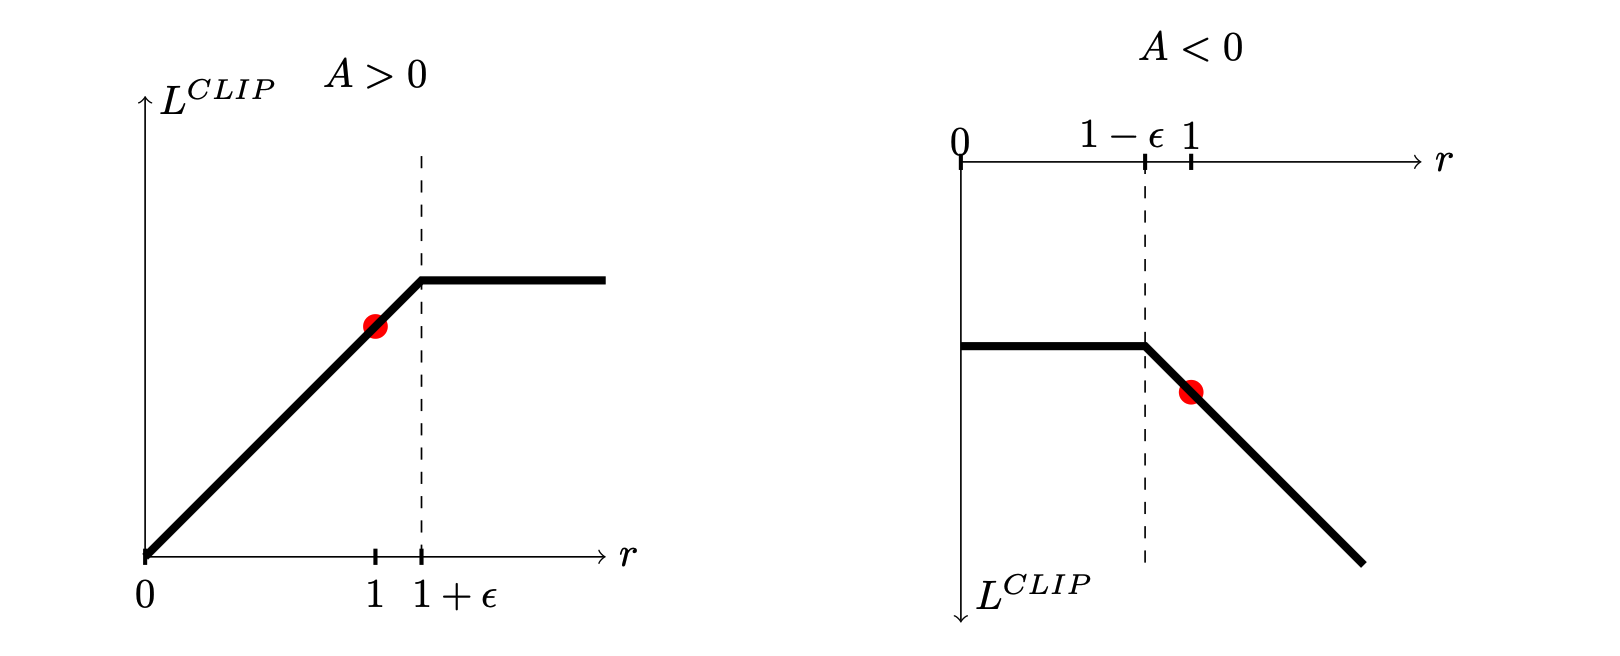
\includegraphics[scale=0.5]{img/ppo_clip.png}
  \caption{PPO Clip Funktion \protect\cite{schulman2017proximal}}
  \label{fig:ppo_clip}
\end{figure}

\begin{lstlisting}[caption={Codeausschnitt von Akteur Verlustfunktion aus Open Ai Spinning Up PPO implementation},captionpos=b]
ratio = torch.exp(logp - logp_old)
clip_adv = torch.clamp(ratio, 1-clip_ratio, 1+clip_ratio) * adv
loss_pi = -(torch.min(ratio * adv, clip_adv)).mean()
\end{lstlisting}

Kritik Verlust Funktion:
Um die Abweichung zwischen der Vorhersage des Kritik Netzes und dem tatsächlichen Ertrag zu messen nutzt PPO die mittlere quadratische Abweichung.
\begin{lstlisting}[caption={Codeausschnitt von Kritik Verlustfunktiion aus Open Ai Spinning Up PPO implementation},captionpos=b]
return ((ac.v(obs) - ret)**2).mean()
\end{lstlisting}
{\chapter{Ml-Agents}}
\label{sec:mlagents}
Das Unity ML-Agents Toolkit ist ein Open-Source-Projekt, in dem maschinelle Lernalgorithmen und Funktionen für die Verwendung mit der Spieleumgebung Unity implementiert und kontinuierlich weiterentwickelt werden. Die Implementierung ist in zwei Bereiche unterteilt. Für die Unity-Integration ist das Paket com.unity.ml-agents aus dem Unity Asset Store zuständig. Das eigentliche Training mit den maschinellen Lernalgorithmen findet jedoch in einer separaten Python-Umgebung statt. Für die Kommunikation zwischen den beiden Bereichen verwendet das ML-Agents Toolkit eine C\# Kommunikator-Klasse, die über gRPC-Netzwerkkommunikation mit dem Python-Prozess kommuniziert. Der Python-Prozess kommuniziert über die Python Low-Level-API, die die Kommunikation übernimmt und die Befehle an den Trainer weiterleitet.\cite{unity_mlagents_toolkit_overview}

\begin{figure}[H]
  \centering  
  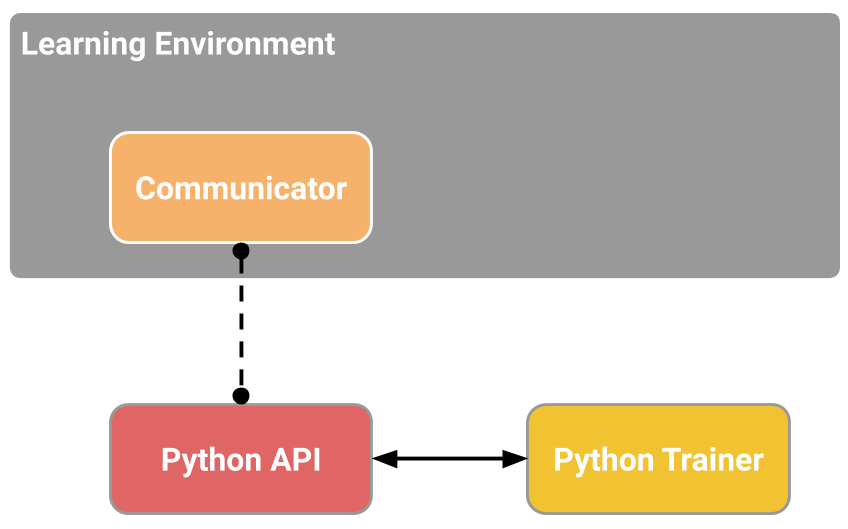
\includegraphics[scale=0.4]{img/learning_environment_basic.png}
  \caption{Unity ML-Agents Lernumgebung \protect\cite{unity_mlagents_learning_environment_basic}}
  \label{fig:learning_environment_basic}
\end{figure}

Das Unity-Paket enthält zwei Komponenten: Agenten und deren Verhalten. Die Agent-Komponente bildet die Grundlage für alle Implementierungen. Sie bietet abstrakte Funktionen für die Initialisierung, den Start einer Episode, das Erfassen des Zustands der Umgebung sowie das Ausführen von Aktionen. Durch die Implementierung dieser Funktionen können unterschiedlichste Agenten entwickelt und trainiert werden. Jeder Agent ist mit einem Verhalten verknüpft, das für jede Beobachtung des Agenten eine Aktion auswählt, die der Agent ausführt. Es gibt drei Arten, wie die Verhaltensweisen agieren können. Im Lernmodus werden die Beobachtungen des Agenten für das Training und die Auswahl einer Aktion anhand des aktuellen Modells verwendet. Der Inferenzmodus nutzt hingegen ein bereits trainiertes Modell und wertet dieses aus. Der letzte Modus eines Verhaltens ist der Heuristikmodus, bei dem festgelegte Regeln im Code entscheiden, welche Aktion ausgeführt wird, ohne die Verwendung eines trainierten Modells.\cite{unity_mlagents_toolkit_overview}

\begin{figure}[H]
  \centering  
  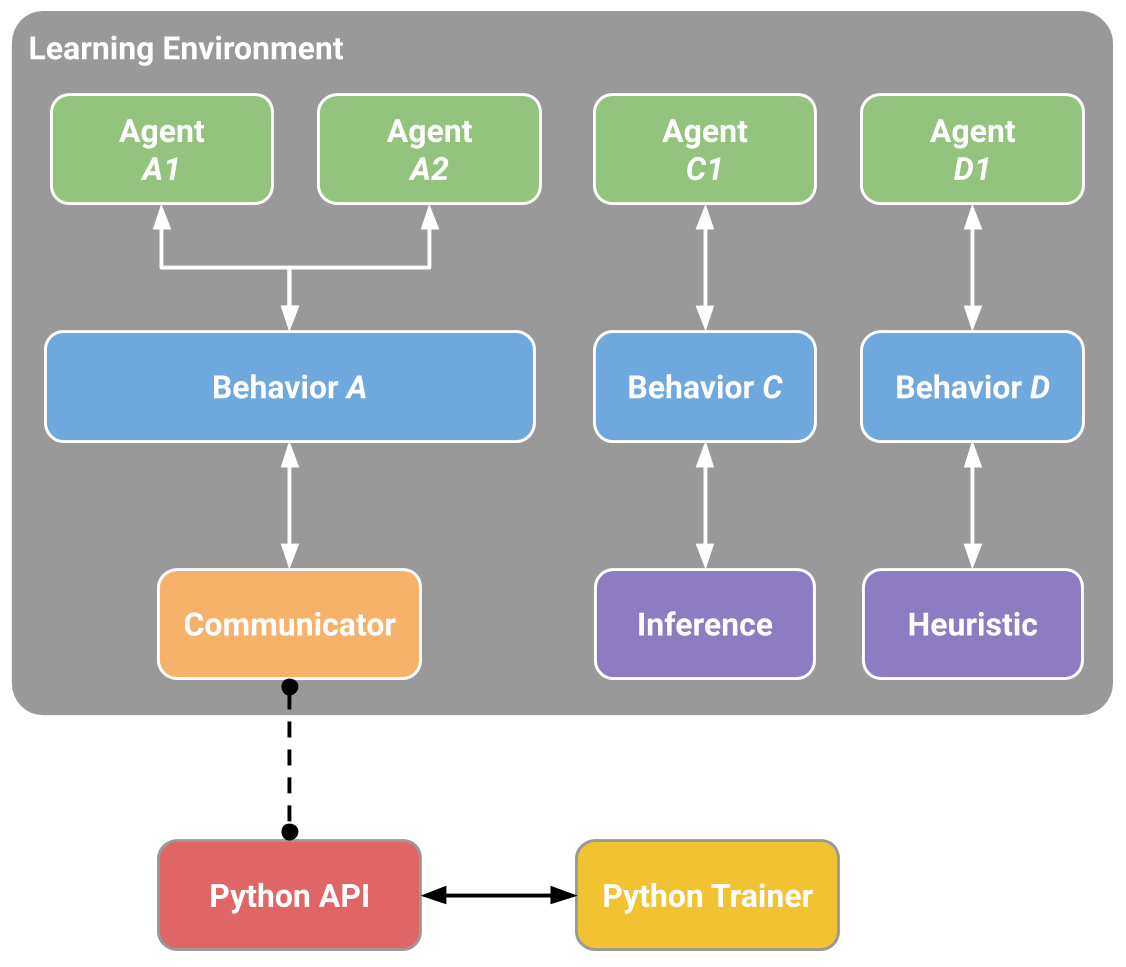
\includegraphics[scale=0.3]{img/learning_environment_example.png}
  \caption{Unity ML-Agents Lernumgebung Beispiel \protect\cite{unity_mlagents_learning_environment_example}}
  \label{fig:learning_environment_example}
\end{figure}

\section{Komponenten}
In diesem Kapitel werde Ich die Grundlegenden Komponenten des Unity ML-Agents Packets, welche in der Arbeit verwendet wurden erklären. Darurch sollten Codeausschnitte und Komponentenabbildungen in folgenden Kapiteln deutlich zu verstehen sein.

\subsection{Verhalten}
\begin{figure}[H]
  \centering  
  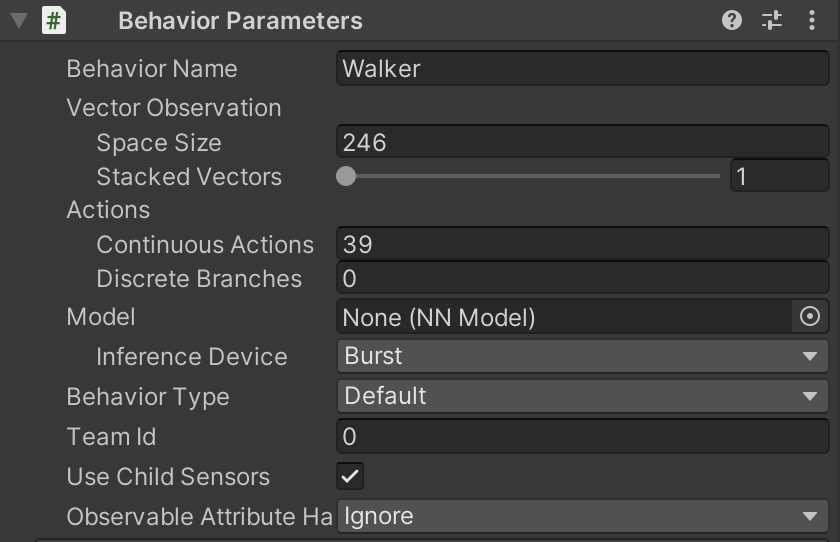
\includegraphics[scale=0.5]{img/verhalten_komponente.png}
  \caption{Unity ML-Agents Verhalten Komponente}
  \label{fig:verhalten_komponente}
\end{figure}

\begin{center}
{\rowcolors{2}{lightgray}{gray!50!lightgray!50}
\begin{tabular}{ |p{4cm}|p{8cm}| }
\hline
Konfigurationsfeld& Beschreibung \\
\hline
Behaviour Name & Name des Verhaltens / wird in Trainer Konfiguration referenziert \\
Space Size & Anzahl an Beobachtungen / Inputknoten für NN \\
Continuous Actions & Anzahl an Aktionen / Outputknoten von NN \\
Model & Referenz auf bereits trainiertes Modell zur Verwendung in Inferenz \\
Behaviour Type & Lernmodus Default = Lernen, Heuristic, Inferenz \\
\hline
\end{tabular}}
\end{center}

\subsection{Entscheidung}
\begin{figure}[H]
  \centering  
  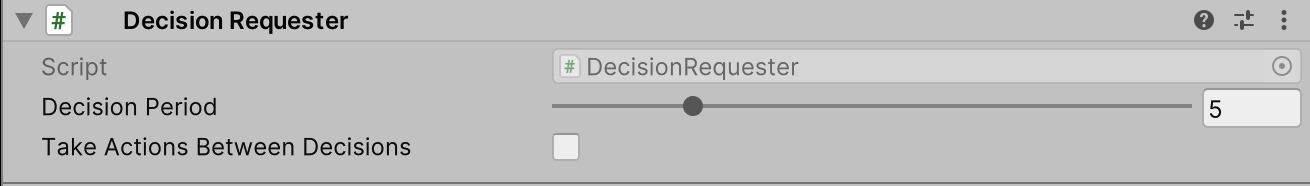
\includegraphics[scale=0.5]{img/entscheidung_anfragen_komponente.png}
  \caption{Unity ML-Agents Entscheidung Anfragen Komponente}
  \label{fig:entscheidung_anfragen_komponente}
\end{figure}

\begin{center}
{\rowcolors{2}{lightgray}{gray!50!lightgray!50}
\begin{tabular}{ |p{4cm}|p{8cm}| }
\hline
Konfigurationsfeld& Beschreibung \\
\hline
Decision Period & Anzahl an Akademie-Schritten (standard ein Schritt pro Physikupdate) bis zur nächsten Entscheidung \\
Take Actions Between Decisions &  Kontrollkasten ob Agent Aktionen zwischen Entscheidungen ausführen soll \\
\hline
\end{tabular}}
\end{center}


\subsection{Agent Abstrakte Funktionen}
Die Akademie stellt mit dem Attribut EnvironmentParameters die Umgebungsparameter aus Trainer Konfiguration oder aktueller Lektion bereit
\begin{lstlisting}
envParams = Academy.Instance.EnvironmentParameters;
\end{lstlisting}

Mit dem StatsRecorder lassen sich Daten aggregieren um diese nach oder während dem Training über die Tensorboard Visualisierung auszuwerten
\begin{lstlisting}
statsRecorder = Academy.Instance.StatsRecorder;
\end{lstlisting}

In der CollectObservations Methoden wird festgelegt welche Daten dem Agent für das Training bereit stehen, dieser Schritt wird für jede angefragte Entscheidung ausgeführt und das Ergebnis an das NN Modell oder den Python Trainer übergeben.
\begin{lstlisting}
public override void CollectObservations(VectorSensor sensor)
{
    sensor.AddObservation(floatObservation);
}
\end{lstlisting}

Wenn eine Entscheidung angefragt wurde und das NN Modell ein Ergebnis liefert wird dieses hier von numerischen Werten in Aktionen umgewandelt.
\begin{lstlisting}
public override void OnActionReceived(ActionBuffers actionBuffers)
{
    var continuousActions = actionBuffers.ContinuousActions;
    float action = continuousActions[0]
}
\end{lstlisting}

Im folgenden Beispielcode wird ein Reward in jedem FixedUpdate vergeben über die AddReward Methode die auch Teil der Agenten-Komponente ist. Der Reward kann aber an jeder Stelle im Code vergeben werden, der Code dient hier nur als ein Beispiel.
\begin{lstlisting}
public virtual void FixedUpdate()
{
    AddReward(floatReward);
}
\end{lstlisting}

Die Trainings Konfigurationdatei enthält mehrere Teile. Der hyperparameter Teil enthält die Hyperparameter des Maschinellen Lernalgorithmuses, danach folgt der network\_settings Teil welcher die Konfiguration des Neuronalennetzes festlegt. Anschließend folgen noch Konfigurationen für die Belohnungssignale im Bereich reward\_signals und Einstellungen für die Speicherung der Daten sowie der länge des Trainings. Ganz am Ende der Konfigurationsdatei befinden sich noch Umgebungsparameter welche erweitert und während dem Training ausgelesen werden können.
\begin{lstlisting}
{
behaviors:
  Walker:
    trainer_type: ppo
    hyperparameters:
      batch_size: 2048
      buffer_size: 20480
      learning_rate: 0.0003
      beta: 0.005
      epsilon: 0.2
      lambd: 0.95
      num_epoch: 3
      learning_rate_schedule: linear
    network_settings:
      normalize: true
      hidden_units: 256
      num_layers: 3
      vis_encode_type: simple
    reward_signals:
      extrinsic:
        gamma: 0.995
        strength: 1.0
    keep_checkpoints: 5
    checkpoint_interval: 5000000
    max_steps: 30000000
    time_horizon: 1000
    summary_freq: 30000
environment_parameters:
  environment_count: 100.0
}
\end{lstlisting}

{\chapter{Analyse}}
\label{sec:analyse}
Zusätzlich zu den maschinellen Lernkomponenten liefert Unity auch Demonstrationsumgebungen, in denen verschiedene Lösungen für gängige Verstärkungslernprobleme implementiert sind. In der Walker-Demo wird ein physisch simulierter Charakter darauf trainiert, zu einem Zielwürfel zu laufen. Diese Demo-Umgebung implementiert bereits einige Grundlagen für die Steuerung eines physisch simulierten Charakters. Aus diesem Grund wird in dieser Arbeit die Walker-Demo als Grundlage für die Entwicklung genutzt. In diesem Kapitel wird daher die Walker-Demo analysiert, um in den folgenden Kapiteln darauf aufzubauen.

\section{Szenenaufbau}

\begin{figure}[H]
  \centering  
  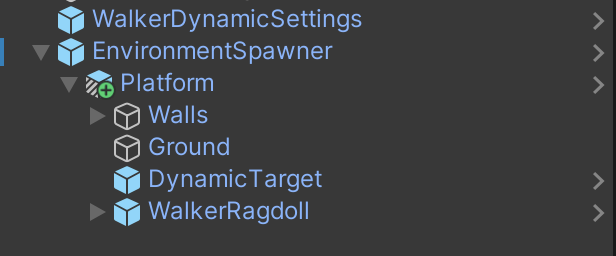
\includegraphics[scale=0.8]{img/walker_demo_hierarchy.png}
  \caption{Walker-Demo Hierarchy}
  \label{fig:walker_demo_hierarchy}
\end{figure}

\begin{figure}[H]
  \centering  
  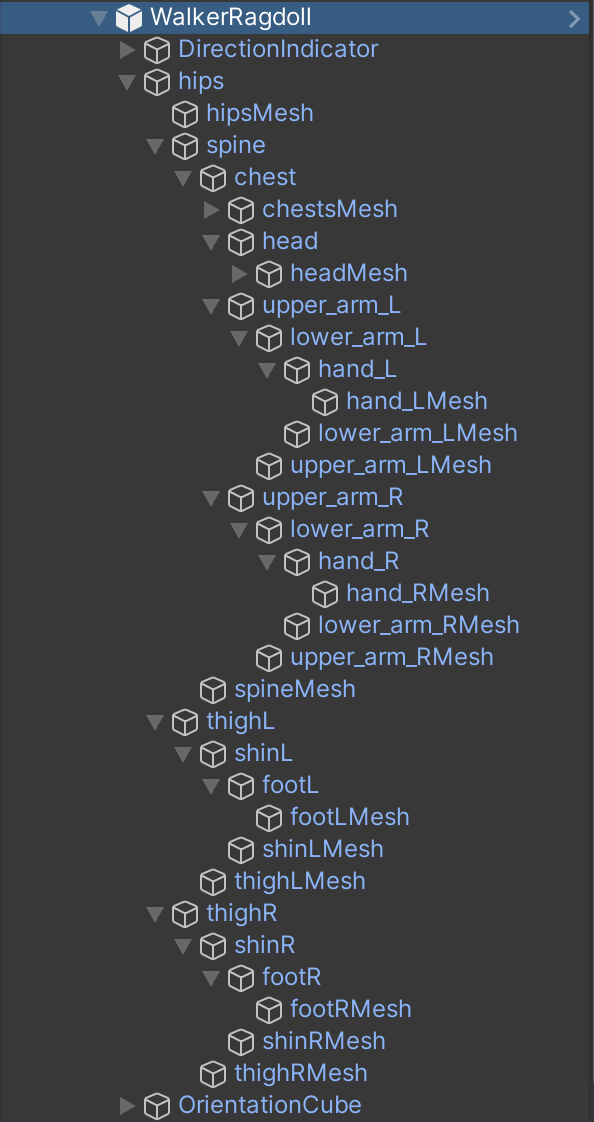
\includegraphics[scale=0.5]{img/agent_hierarchy.png}
  \caption{Agent Hierarchy}
  \label{fig:agent_hierarchy}
\end{figure}


\section{Physikkomponenten und -konfiguration}
Der Körper besteht aus 11 Kapseln, drei Kugeln und 2 Quadern, jeder dieser Formen hat eine Festkörper und eine Kollisions Physikkomponente. Zwischen den Körperteilen werden die Gelenke als Kugelgelenke simuliert.

\begin{center}
{\rowcolors{2}{lightgray}{gray!50!lightgray!50}
\begin{tabular}{ |p{3cm}|p{3cm}|p{2cm}|p{4cm}|p{2cm}| }
\hline
Körperteil& Verbundenes Körperteil & Gewicht & Winkellimits & Form \\
\hline
Hüfte & - & 15kg & - & Kapsel \\
Wirbelsäule & Hüfte & 10kg & x(-20,20) y(-20,20) z(-15,15) & Kapsel \\
Oberkörper & Wirbelsäule & 8kg & x(-20,20) y(-20,20) z(-15,15) & Kapsel \\
Kopf & Oberkörper & 6kg & x(-30,10) y(-20,20) & Kugel \\
Oberarm LR & Oberkörper & je 4kg & x(-60,120) y(-100,100) & Kapsel \\
Unterarm LR & Oberarm & je 3kg & x(0,160) & Kapsel \\
Hand LR & Unterarm & je 2kg & - & Kugel \\
Oberschenkel LR & Hüfte & je 14kg& x(-90,60) y(-40,40) & Kapsel \\
Unterschenkel LR & Oberschenkel & je 7kg &  x(0,120) & Kapsel \\
Fuß LR & Unterschenkel & je 5kg & x(-20,20 y(-20,20) z(-20,20) & Quader \\
\hline
\end{tabular}}
\end{center}

\section{Agent implementierung}
lernablauf (Beobachtung, Aktionen ausführen, Belohnungsfunktion, einrichtung)

\begin{figure}[H]
  \centering  
  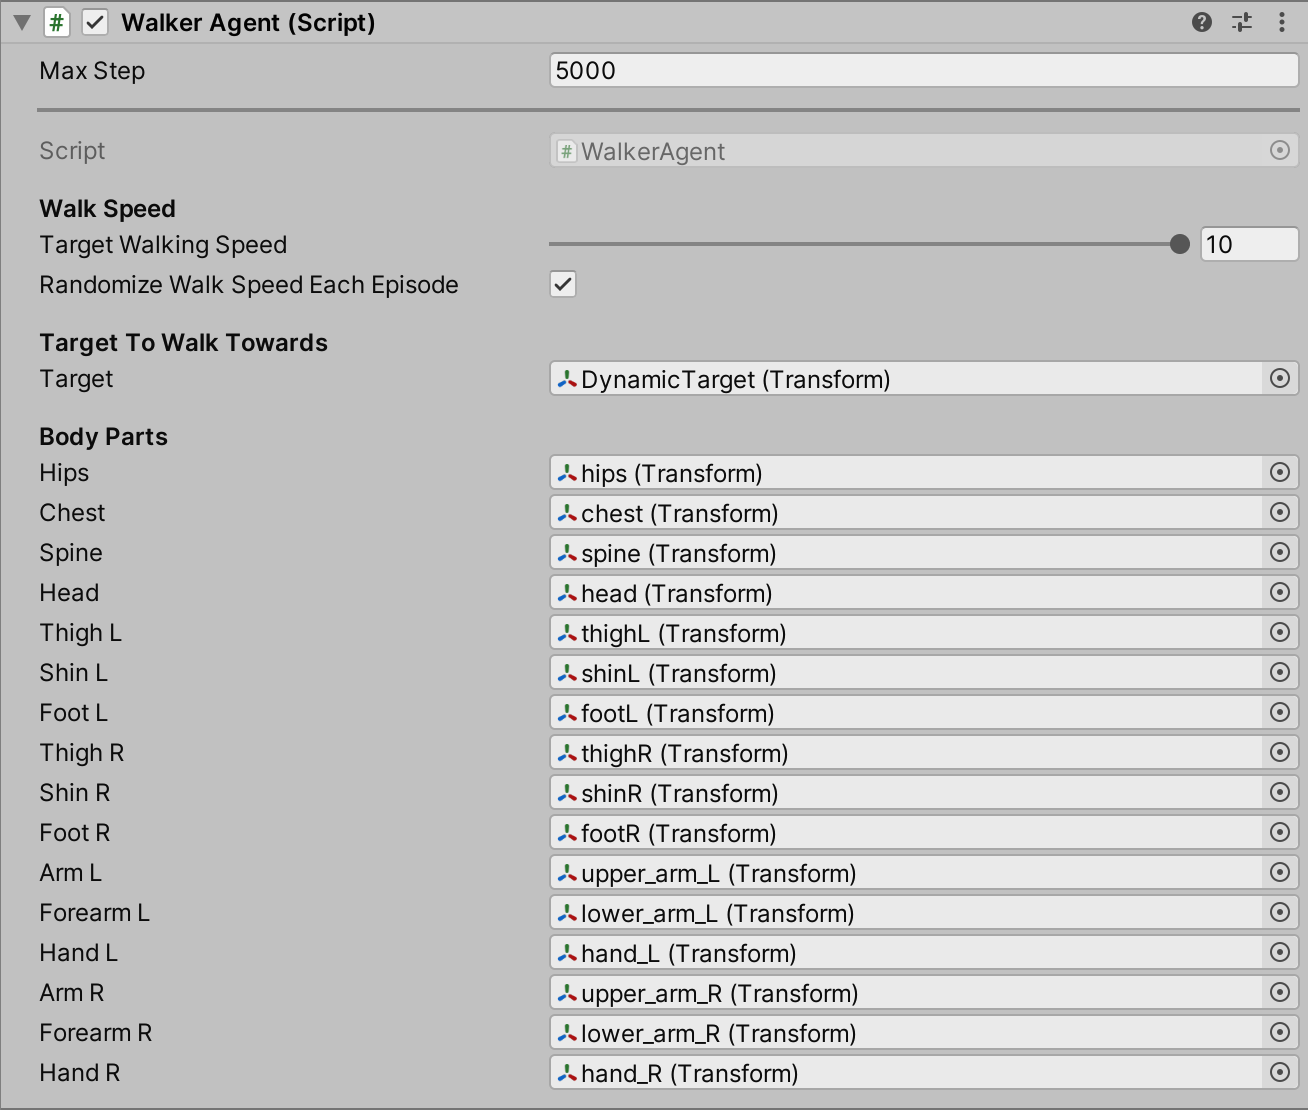
\includegraphics[scale=0.5]{img/agent_konfiguration.png}
  \caption{Agent Konfiguration}
  \label{fig:agent_konfiguration}
\end{figure}

Agent Code hier einfügen? oder evtl. im Anhang?

\section{Ziel}
Ziele (target controller)
{\chapter{Fazit}}
\label{sec:fazit}
Text

\appendix
\chapter{Anhang 1}

%Literaturverzeichnis
\printbibliography[title=Literaturverzeichnis]

\end{document}
